\section*{2.6 电路}
电路理论是一个重要的应用,它自然会导致线性方程组的矩形系统。由于基础数学依赖于前面几节讨论的几个概念,你可能会发现对电路进行初等数学分析是一次有趣且值得的探索。然而,省略本节不会影响文本的连续性。

在包含电阻和电动势(EMF)源(如电池)的直流电路中,三个或更多导体连接的点称为电路的节点或分支点,闭合的传导路径称为回路。电路中两个相邻节点之间的任何部分称为支路。图2.6.1所示的电路是一个典型示例,包含四个节点、七个回路和六个支路。

\begin{figure}[h]
    \centering
    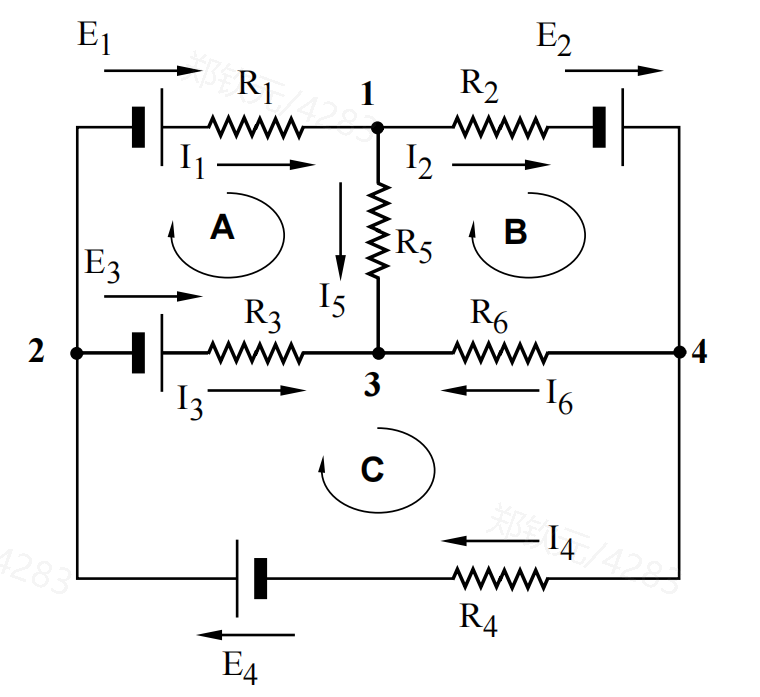
\includegraphics[width=\linewidth]{fig2.6.1} 
    \caption{图2.6.1}
    \label{fig:2.6.1}
\end{figure}

问题是将每个支路中的电流 \(I_k\) 与电阻 \(R_k\) 和电动势 \(E_k\) 联系起来。这可以通过使用欧姆定律结合基尔霍夫定律来产生线性方程组来实现。

\begin{bluebox}{欧姆定律}
欧姆定律指出:对于电流 \(I\) 安培,电阻 \(R\) 欧姆上的电压降(单位:伏特)为 \(V = IR\)。

对于大小为 \(E\) 的EMF源和电流 \(I\),源内部总是有一个小的内阻,其上的电压降为 \(V = E - I \times \text{内阻}\)。但内阻通常可忽略,因此源上的电压降可视为 \(V = E\)。当内阻不可忽略时,其效应可以合并到现有外部电阻中,或视为单独的外部电阻。
\end{bluebox}

\begin{bluebox}{基尔霍夫定律}
\textbf{节点规则:} 流向每个节点的电流的代数和为零。即,总流入电流必须等于总流出电流。这仅仅是电荷守恒的陈述。

\textbf{回路规则:} 每个回路中电动势的代数和必须等于同一回路中 \(IR\) 乘积的代数和。即,假设源内阻已考虑,则源上电压降的代数和等于每个回路中电阻上电压降的代数和。这是能量守恒的陈述。
\end{bluebox}

基尔霍夫定律可以在不知道电流和EMF方向的情况下使用。你可以任意指定方向。如果最终解中出现负值,则实际方向与假设方向相反。应用节点规则时,如果电流方向朝向节点,则视为正;否则视为负。显然,节点规则总是产生齐次方程组。例如,将节点规则应用于图2.6.1中的电路,会产生四个齐次方程,六个未知数(即 \(I_k\)):
\[
\begin{aligned}
&\text{节点1: } I_1 - I_2 - I_5 = 0 \\
&\text{节点2: } I_2 - I_3 - I_4 = 0 \\
&\text{节点3: } I_5 + I_6 - I_1 = 0 \\
&\text{节点4: } I_3 + I_4 - I_6 = 0
\end{aligned}
\]

应用回路规则时,必须选择某个方向(顺时针或逆时针)作为正方向,该方向上的所有EMF和电流视为正,相反方向视为负。一个电流在节点规则中可能被视为正,但在回路规则中使用时可能被视为负。如果正方向被视为顺时针,则将回路规则应用于图2.6.1中的三个指示回路A、B和C,会产生三个非齐次方程,六个未知数(\(I_k\) 视为未知数,而 \(R_k\) 和 \(E_k\) 假设已知):
\[
\begin{aligned}
&\text{回路A: } E_1 - E_2 = I_1 R_1 - I_2 R_2 \\
&\text{回路B: } E_2 = I_2 R_2 + I_3 R_3 + I_4 R_4 \\
&\text{回路C: } E_3 = I_4 R_4 - I_5 R_5 - I_6 R_6
\end{aligned}
\]

还有另外四个回路也会产生回路方程,总共有11个方程(4个节点方程和7个回路方程)和6个未知数。虽然这看起来是一个一般的 \(11 \times 6\) 方程组,但事实并非如此。如果电路处于平衡状态,则物理情况要求对于每组EMF \(E_k\),对应的电流 \(I_k\) 必须唯一确定。换句话说,物理保证由基尔霍夫定律产生的 \(11 \times 6\) 系统必须是一致的且具有唯一解。

假设 \([A \mid b]\) 表示由基尔霍夫定律生成的 \(11 \times 6\) 系统的增广矩阵。从 §2.5 的结果中,我们知道系统有唯一解当且仅当:
\[
\text{rank}(A) = \text{rank}([A \mid b]) = n = 6
\]
此外,§2.3 中证明了系统是一致的当且仅当:
\[
\text{rank}(A) = \text{rank}([A \mid b])
\]
结合这两个事实,我们可以得出结论:
\[
\text{rank}([A \mid b]) = \text{rank}(A) = 6
\]
因此,当 \([A \mid b]\) 被简化为 \(E_{[A \mid b]}\) 时,将恰好有6个非零行和5个零行。因此,原始11个方程中有5个是冗余的,因为它们可以通过特定6个“独立”方程的组合“归零”。最好提前知道11个方程中哪些是冗余的,哪些可以作为“独立”集。

注意,在使用节点规则时,节点4的方程仅仅是节点1、2和3方程的负和,且前三个方程是独立的,即三个方程中没有一个可以写为其他两个的组合。这种情况是典型的。对于具有 \(n\) 个节点的一般电路,可以证明前 \(n-1\) 个节点的方程是独立的,最后一个节点的方程是冗余的。

回路规则也会产生冗余方程。只有简单回路(不包含更小回路的回路)会产生独立方程。例如,考虑图2.6.1中由三个外部支路组成的大回路。将回路规则应用于这个大回路不会产生新信息,因为大回路可以通过“加”其内部的三个简单回路A、B和C来构造。与大外部回路相关的方程为:
\[
E_1 - E_2 + E_3 = I_1 R_1 - I_2 R_2 + I_3 R_3 + I_4 R_4 - I_5 R_5 - I_6 R_6
\]
这正好是对应三个组成回路A、B和C的方程之和。这种现象在一般情况下成立,因此使用回路规则时只需考虑简单回路。

讨论的要点是结论:更一般的 \(11 \times 6\) 矩形系统可以通过丢弃最后一个节点方程并仅使用简单回路方程,替换为等效的 \(6 \times 6\) 平方系统,该系统具有唯一解。这是实际工作的典型特征。问题的物理性质连同自然约束通常可用于将一般矩形系统替换为平方且具有唯一解的系统。

我们研究的目标之一是更清楚地理解此应用中出现的“独立性”概念。到目前为止,独立性是一个直观概念,但此示例有助于阐明独立性是一个基本重要概念,值得更牢固地确定。这将在§4.3中完成,并且从电路获得独立方程的一般理论在示例4.4.6和4.4.7中开发。

\textcolor{red}{练习2.6}
\color{red}\rule{\textwidth}{0.4pt}\color{black}

\begin{enumerate}[leftmargin=*, label=\bfseries 2.6.\arabic*]
    \item 假设在图2.6.1所示的电路中,\(R_i = i\) 欧姆,\(E_i = i\) 伏特。
    \begin{enumerate}[label=(\alph*)]
        \item 确定六个指示电流。
        \item 选择节点1作为参考点,并将其电位固定为0伏特。相对于此参考,计算其他三个节点的电位。通过验证每个回路的回路规则来检查你的答案。
    \end{enumerate}

    \item 确定以下电路中的三个指示电流。
    \begin{figure}[h]
        \centering
        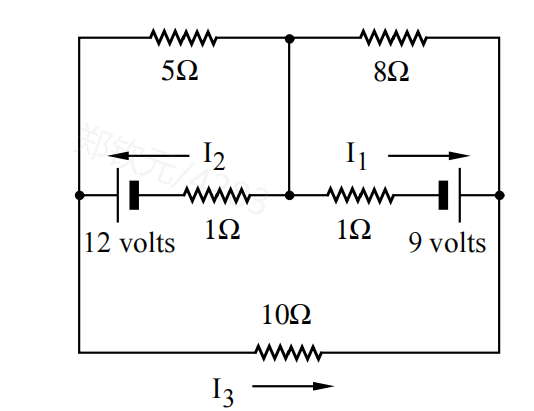
\includegraphics[width=\linewidth]{fig2.6.2} 
        \caption{图2.6.2}
        \label{fig:2.6.2}
    \end{figure}

    \item 确定以下电路中的两个未知EMF。
    \begin{figure}[h]
        \centering
        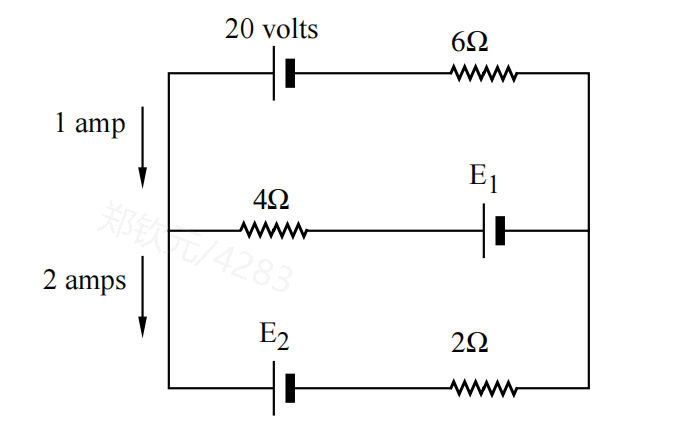
\includegraphics[width=\linewidth]{fig2.6.3} 
        \caption{图2.6.3}
        \label{fig:2.6.3}
    \end{figure}

    \item 考虑以下所示电路并回答以下问题。
    \begin{figure}[h]
        \centering
        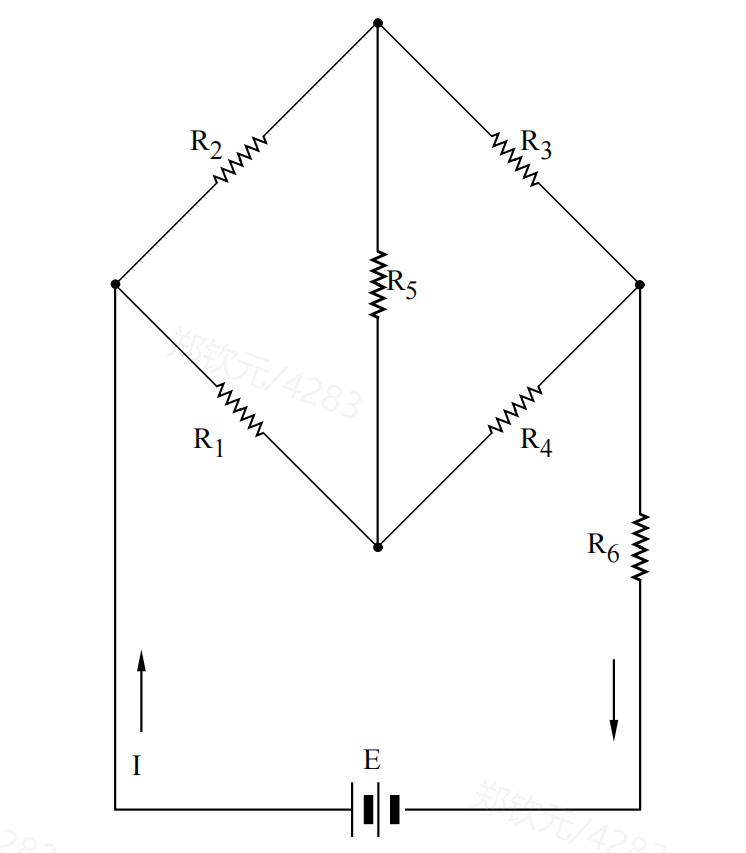
\includegraphics[width=\linewidth]{fig2.6.4} 
        \caption{图2.6.4}
        \label{fig:2.6.4}
    \end{figure}
    \begin{enumerate}[label=(\alph*)]
        \item 电路包含多少个节点?
        \item 电路包含多少个支路?
        \item 确定回路的总数,然后确定简单回路的数量。
        \item 证明简单回路方程形成“独立”方程组,即没有冗余方程。
        \item 验证任何三个节点方程构成“独立”方程组。
        \item 验证与包含 \(R_1, R_2, R_3, R_4\) 的回路相关的回路方程可以表示为包含在较大回路中的两个简单回路的两个方程之和。
        \item 如果 \(R_1 = R_2 = R_3 = R_4 = 1\) 欧姆,\(R_5 = R_6 = 5\) 欧姆,且 \(E = 5\) 伏特,确定指示电流 \(I\)。
    \end{enumerate}
\end{enumerate}
